\documentclass[11pt,xcolor=svgnames]{beamer}
\usepackage{dsfont,natbib,setspace,changepage,multirow}
\mode<presentation>

% fonts

% replaces beamer foot with simple page number
\setbeamertemplate{navigation symbols}{}
\setbeamercolor{frametitle}{fg=black}
\setbeamerfont{frametitle}{series=\bfseries}
\setbeamerfont{frametitle}{size=\normalsize}

\newcommand{\theme}{\color{Maroon}}

\setbeamertemplate{footline}{
   \raisebox{5pt}{\makebox[\paperwidth]{\hfill\makebox[20pt]{\color{gray}\scriptsize\insertframenumber}}}}

\graphicspath{{../graphs/}}

%\setbeamercolor{whitebox}{bg=gray!10}

% colors
\newcommand{\bk}{\color{black}}
\newcommand{\rd}{\color{red}}
\newcommand{\fg}{\color{ForestGreen}}
\newcommand{\bl}{\color{blue}}
\newcommand{\gr}{\color{black!60}}
\newcommand{\sg}{\color{DarkSlateGray}}
\newcommand{\br}{\color{SaddleBrown}}
\newcommand{\nv}{\color{Navy}}
\setbeamercolor{itemize item}{fg=gray}

% common math markups
\newcommand{\bs}[1]{\boldsymbol{#1}}
\newcommand{\mc}[1]{\mathcal{#1}}
\newcommand{\mr}[1]{\mathrm{#1}}
\newcommand{\bm}[1]{\mathbf{#1}}
\newcommand{\ds}[1]{\mathds{#1}}
\newcommand{\indep}{\perp\!\!\!\perp}

% spacing and style shorthand
\setstretch{1.1}

% shorthand
\newcommand{\sk}{\vspace{.5cm}}
\newcommand{\R}[1]{{\tt \nv #1}}
\newcommand{\til}{{\footnotesize$\bs{\stackrel{\sim}{}}$}}
\DeclareSymbolFont{extraup}{U}{zavm}{m}{n}
\DeclareMathSymbol{\vardiamond}{\mathalpha}{extraup}{87}

\begin{document}

\setcounter{page}{0}
{ \usebackgroundtemplate{
\includegraphics[height=\paperheight]{phoenix}}
\begin{frame}[plain]
\begin{center}


{\bf \Large [3] Big Data: Model Selection }

\vskip 1.5cm 
Matt Taddy, University of Chicago Booth School of Business

\vskip .2cm 
\texttt{faculty.chicagobooth.edu/matt.taddy/teaching} 


\end{center}
\end{frame} }

%\setbeamercolor{background canvas}{bg=gray!10}

\begin{frame}
{[3] \theme  Making Model Decisions}

Out-of-Sample vs In-Sample performance

\vskip .5cm 
Regularization paths and the lasso

\vskip .5cm 
OOS experiments and Cross Validation

\vskip .5cm
Information Criteria
\begin{itemize}
\item AIC and the corrected AICc
\item BIC and Bayesian model selection
\end{itemize}

\end{frame}

\begin{frame}
{Some basic facts about linear models}

{The model is always $\ds{E}[y|\bm{x}] = f(\bm{x}\bs{\beta})$.}
\begin{itemize}
\item Gaussian (linear): $y \sim \mr{N}(\bm{x}\bs{\beta},\sigma^2)$. 
\item Binomial (logistic): $\mr{p}(y=1)= e^{\bm{x}\bs{\beta}}/(1+ e^{\bm{x}\bs{\beta}})$.
\end{itemize}

\vskip .4cm
{\nv LHD($\bs{\hat\beta}$) and dev($\bs{\hat\beta}$): }

\vskip .2cm
Likelihood (LHD) is $\mr{p}(y_1|\bm{x}_1)\times\mr{p}(y_2|\bm{x}_2)\cdots\times\mr{p}(y_n|\bm{x}_n)$.

\vskip .2cm
The Deviance (dev) is proportional to -log(LHD).

\vskip .2cm
$\bs{\hat\beta}$ is commonly fit to maximize LHD $\Leftrightarrow$ minimize deviance.

\vskip .5cm
Fit is summarized by $R^2 = 
1 - \text{dev}(\bs{\hat\beta})/\text{dev}(\bs{\beta}=0)$.

\vskip .2cm

{\theme The only $R^2$ we ever really care about is out-of-sample $R^2$.}

\end{frame}

\begin{frame}

The $R^2$ is always $1 - \text{dev}(\bs{ \hat \beta})/\text{dev}(\bs{\beta}=\bm{0})$.  

\vskip .1cm
The difference between {\it in} and {\it out} of sample $R^2$ is what data are used to fit $\bs{ \hat \beta}$ and what the deviances are calculated on.

\vskip .5cm
For {\theme in-sample} $R^2$, we have data $[\bm{x}_1,y_1] \ldots [\bm{x}_n, y_n]$ and you  use this data to fit
$\bs{ \hat \beta}$.  The deviance is then, say for linear regression,
\[
\text{dev}(\bs{ \hat \beta}) = \sum_{i=1}^n (y_i - \bm{x}_i'\bs{\hat\beta})^2
\]

For {\theme out-of-sample} $R^2$, observations $1...n$ are still used to fit $\bs{ \hat \beta}$ but the deviance is now caluclated over {\textit new} observations, say
\[
\text{dev}(\bs{ \hat \beta}) = \sum_{i=n+1}^{n+m} (y_i - \bm{x}_i'\bs{\hat\beta})^2
\]
\vskip -.5cm
\end{frame}

\begin{frame}
{{\nv Example:} Semiconductor Manufacturing Processes}

\begin{columns}[c]

\column{1.75in}

\vskip .25cm

\includegraphics[width=2in]{schalfhigh}
\column{2in}\small
\begin{center}


Very complicated operation\\
{\sg Little margin for error.}


\vskip .25cm
Hundreds of diagnostics\\
{\sg Useful or debilitating?}

\vskip .25cm
We want to focus reporting and
better predict failures.

\end{center}

\end{columns}

\sk
$\bm{x}$ is 200 input signals, $y$ has 100/1500 failures.

\vskip .25cm
Logistic regression for failure of chip $i$ is

\vspace{-.25cm}
\[p_i = \mr{p}({\tt fail}_i|\bm{x}_i) = e^{\alpha+\bm{x}_i\bs{\beta}}/(1+ e^{\alpha+\bm{x}_i\bs{\beta}})
\]


% The $x_{ij}$ inputs here are actually orthogonal: they are the first 200 Principal Component directions from an even bigger set.

\vspace{-.25cm}

\end{frame}

\begin{frame}
{Semiconductor FDR Control}

The full model has $R^2 = 0.56$ {\gr (based on {\it binomial} deviance)}.

The p-values for these 200 coefficients:


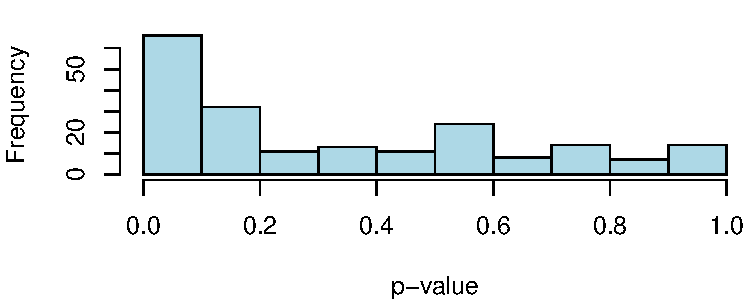
\includegraphics[width=4.1in]{../graphs/SCpvals}

\vskip .25cm

{\gr Some are clustered at zero, the rest sprawl out to one.}\\

FDR of $q=0.1$ yields  $\alpha=0.0122$ p-value rejection cut-off. \\Implies 25 `significant', of which approx 22-23 are true signals.

\end{frame}


\begin{frame}
{semiconductors}

A {\it cut} model, using only these 25  signals,
has $R_{cut}^2 = 0.18$.  \\
This is much smaller than the full model's $R_{full}^2=0.56$.

\sk
In-Sample (IS) $R^2$ {\it always} increases with more covariates.
\\ {\gr This is exactly what MLE $\bs{\hat\beta}$ is fit to maximize.}
\\ {\theme But how well does each model predict {\it new} data?}

\sk
{ An out-of-sample (OOS) experiment}
\begin{itemize}
\item split the data into 10 random subsets {(`folds')}.
\item Do 10x: fit model $\bs{\hat\beta}$ using only 9/10 of data, 
\\ ~~~~~~~~~~~and record $R^2$ on the left-out subset. 
\end{itemize}
These OOS $R^2$ give us a sense of how well each \\model can predict
data that it has not already seen.
\end{frame}

\begin{frame}
{OOS experiment for semiconductor failure}

We gain predictive accuracy by {\it dropping} variables.

\begin{center}\vspace{-.2cm}
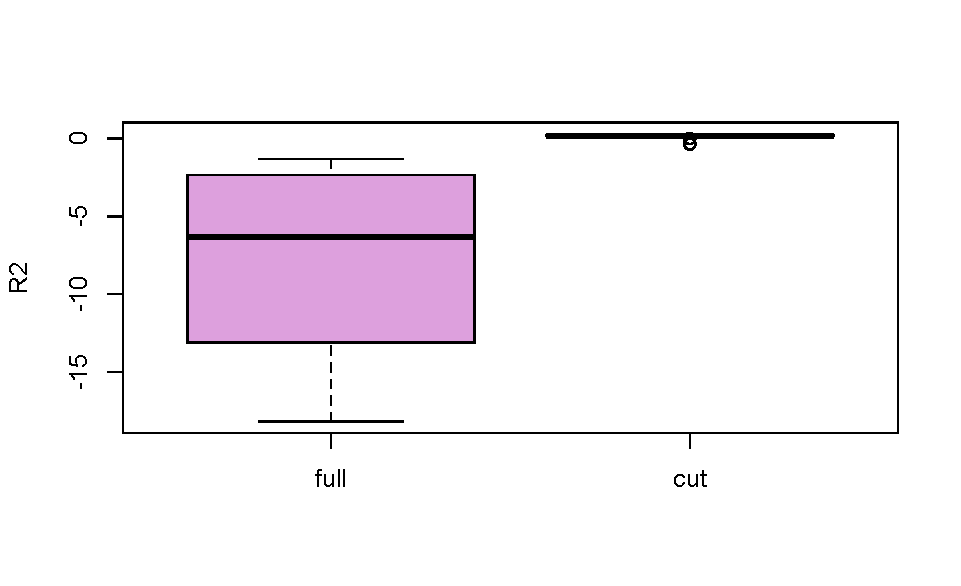
\includegraphics[width=4in]{SCr2}
\end{center}

Cut model has mean OOS R2 of 0.09, about 1/2 in-sample R2.

\vskip .2cm
The full model is terrible.  It is overfit and worse than $\bar y$.\\ 
{\nv Negative R2 are more common than you might expect.}

\vspace{-.2cm}
\end{frame}

\begin{frame}
{OOS experimentation}

{\nv All that matters is Out-of-Sample $R^2$.}  \\{\theme We don't care about In Sample $R^2$.}

\sk
Using OOS experiments to  choose the best model is called {\it cross validation}.  It will be a big part of our big data lives.

\sk
Selection of `the best' model is at the core of all big data.

\vskip .1cm
But before getting to selection, we first need strategies to \\ build good sets of candidate models to choose amongst.

\end{frame}



\begin{frame}
{FDR as a selection tool?}

A heretical way to think about `$\nv q$': a tuning parameter?

\vskip .1cm
Maybe we grab models for $q=0.1,0.2,\ldots$ and compare?


\sk
{\nv Problems with testing/FDR:}

\vskip .2cm
FDR theory requires {\it independence between tests}.  This almost never holds.
In regression, multicollinearity causes problems.
{\gr Given two highly correlated $x$'s you're unsure which to use.\\
You then get big p-values and neither variable is significant.}

\vskip .2cm
Regression $p$-values are based on the full model.  This is probably a terrible model.
{\gr e.g., $p$-values only exist for $p<n$.}

\end{frame}


\begin{frame}
{\theme Forward stepwise regression}

\vskip .25cm
Forward stepwise procedures: start from a simple `null' model, 
and incrementally update fit to allow slightly more complexity.

\vskip .25cm
{\nv Better than backwards methods}
\begin{itemize}
\item The `full' model can be expensive or tough to fit, 
while the null model is usually available in closed form.
\item Jitter the data and the full model 
can change dramatically (because it is overfit).  The null model is always the same.
\end{itemize}

\vskip .25cm
Stepwise approaches are `greedy': they find the best solution at each step 
without thought to global path properties.  


\end{frame}


\begin{frame}
{Naive forward stepwise regression}

\vskip .25cm
The {\tt \nv step()} function in R executes a common routine:

\vskip .05cm
\begin{itemize}
\item Fit all univariate models.  
Choose that with highest (IS) $R^2$ \\
 and put that variable -- say $x_{(1)}$ -- in your model.
\item Fit all bivariate models including $x_{(1)}$ 
($y \sim \beta_{(1)}x_{(1)} + \beta_jx_j$), 
and add $x_j$ from one with highest $R^2$ to your model.
\item Repeat:  max $R^2$ by adding one variable to your  model.
\end{itemize}

\vskip .05cm
You stop when some model selection rule (AIC) is lower for the
current model than for any of the models that add one variable.

\end{frame}

\begin{frame}[fragile]
{Forward stepwise regression in R}

{Easiest way to {\tt \nv step()}: run {\theme null} and {\theme full}
regressions.}
{\nv \small
\begin{verbatim}
null = glm(y ~ 1, data=D)
full = glm(y ~ ., data=D)
fwd = step(null, scope=formula(full), dir="forward")
\end{verbatim}}

{\tt  \nv scope} is the biggest possible model.\\
Iterate for interactions: {\nv\small\verb! fwd2 = step(fwd, scope=.^2, ...!}

\sk
{\bf\gr Example: semiconductors...}

\end{frame}

\begin{frame}
{The problem with Subset Selection}


{\tt \nv step()} is very slow {\gr (e.g., 90 sec for tiny semiconductors)}

\vskip .5cm
This is true in general with {\theme subset selection} (SS): 

\vskip .1cm
Enumerate candidate models by applying maximum likelihood estimation for subsets of coefficients, with the rest set to zero.

\vskip .5cm
SS is slow because adding one variable to a regression can change fit dramatically: {\it each model must be fit from scratch}.

\vskip .5cm
A related subtle (but massively important) issue is {\theme stability}.

\vskip .1cm MLEs have high {\it sampling variability}: they change a lot from one dataset to another.  So which MLE model is `best' changes a lot.

\vskip .1cm $\Rightarrow$  predictions based upon the `best' model will be have high variance.   And big variance leads to big expected errors.

\end{frame}



\begin{frame}
{Regularization}

The key to contemporary statistics is
{\nv regularization:} \\~~~~~~~~~~~~~~~depart from optimality to stabilize a system.

{\gr Common in engineering: I wouldn't drive on an optimal bridge.}

\vskip .5cm
We minimize deviance \onslide<2->{{\nv plus a cost on the size of
coefficients.}} {\large\begin{equation*}
\mr{min} 
-\frac{2}{n}\log \text{LHD}(\bs{\beta}) 
\onslide<2->{{\nv + \lambda\sum_k |\beta_k|}}
\end{equation*}}

\vskip -.25cm
\onslide<2>{This particular cost gives the `lasso': the new least squares.}

\end{frame}


\begin{frame}
{Decision theory: \theme Cost in Estimation}


Decision theory is based on the idea that choices have costs.\\
Estimation and hypothesis testing: what are the costs?


\sk 
{\nv Estimation:}

\vskip .1cm
Deviance is the cost of distance between data and the model.\\
{\gr Recall: $\sum_i (y_i-\hat{y}_i)^2$ or 
$-\sum_i y_i\log(\hat{p}_i) - (1-y_i )\log(1-\hat{p}_i)$.}

\vskip .25cm
{\nv Testing:}

\vskip .1cm
Since $\hat{\beta}_j = 0$ is  {\it safe},  it should cost us to
decide otherwise.

\sk 
$\Rightarrow$ The cost of $\hat{\beta}$ is deviance plus
a penalty  away from zero.



\end{frame}


\begin{frame}
{{\gr [Sparse]}  Regularized Regression}


{\nv\large\[
\mr{min} \left\{ -\frac{2}{n}\log\text{LHD}(\bs{\beta}) + \lambda \sum_j c(\beta_j)\right\}
\]}

$\lambda >0$ is the penalty weight, $c$ is a cost (penalty) function.

$c(\beta)$ will be lowest at $\beta=0$ and we pay more for $|\beta| > 0$.

\vskip .1cm
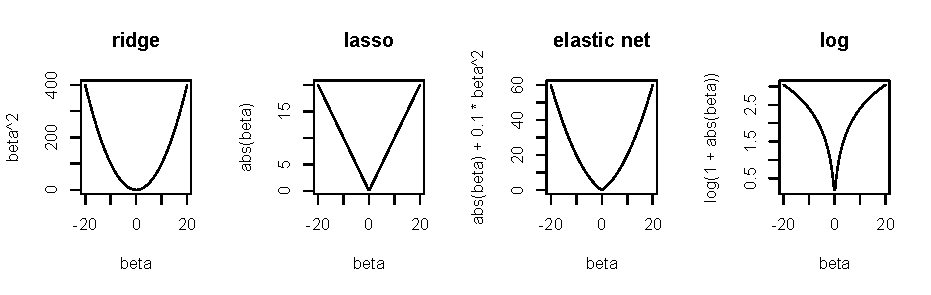
\includegraphics[width=4.25in]{penalties}

Options: ridge $\beta^2$, lasso $|\beta|$, elastic net $\alpha\beta^2 + |\beta|$,  $\log(1 + |\beta|)$.


\end{frame}


\begin{frame}
{Penalization can yield {\theme automatic variable selection}}

The minimum of a smooth + pointy function can be at the point.

\vskip -.25cm
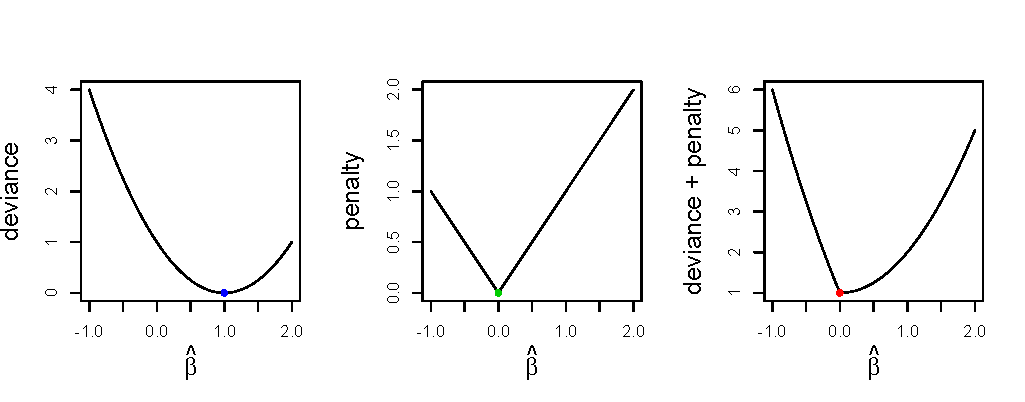
\includegraphics[width=4.25in]{penlasso}

\vskip .5cm
Anything with an absolute value (e.g., lasso) will do this.  

\vskip .1cm 
{\gr There are MANY penalty options and far too much theory.}

\vskip .1cm 
Think of lasso as a baseline, and others as variations on it.

\end{frame}

\begin{frame}
{Lasso Regularization Paths}


The lasso fits $\bs{\hat\beta}$ to minimize $-\frac{2}{n}\log\text{LHD}(\bs{\beta}) + \lambda \sum_j |\beta_j|$.

\vskip .1cm
We'll do this for a {\it sequence} of penalties $\lambda_1 > \lambda_2 ... > \lambda_T$.

\vskip .1cm
{\gr Then we can apply model selection tools to choose best $\hat \lambda$.}

\sk
{\nv Path estimation:}

\vskip .1cm
~~~ Start with big $\lambda_1$ so big that $\bs{\hat \beta}=\bm{0}$.

\vskip .1cm
~~~ For $t=2\ldots T$: update $\bs{\hat \beta}$ to be optimal under $\lambda_t < \lambda_{t-1}$.

\sk


Since estimated $\bs{\hat\beta}$ changes smoothly along this path:
\begin{itemize}
\item It's fast!  Each update is easy.
\item It's stable: optimal $\lambda_t$ may change a bit from sample to sample, but that won't affect the model much.
\end{itemize}
{\gr It's a better version of forward stepwise selection.}

\end{frame}


\begin{frame}
{Path plots}

\vskip .25cm
The whole enterprise is easiest to understand visually.

\vskip -.25cm
\begin{center}
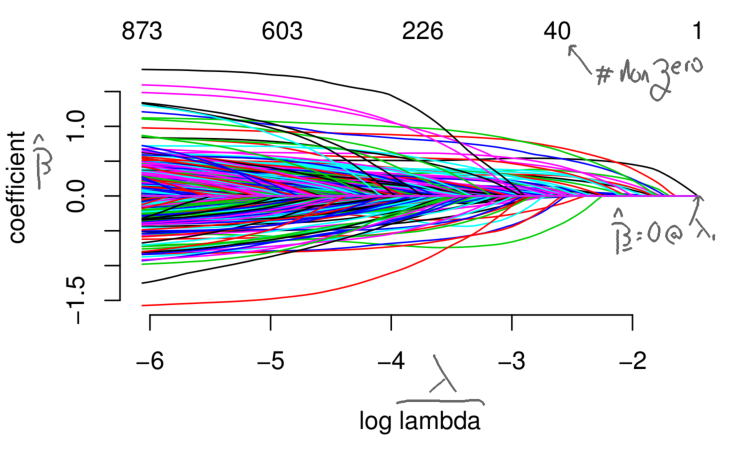
\includegraphics[width=.95\textwidth]{comscore_markeduppaths}
\end{center}

\vskip -.25cm
The algorithm moves {\it right to left}.  \\The $y$-axis is $\bs{\hat\beta}$ (each line a different $\hat\beta_j$) as a function of $\lambda_t$.
\end{frame}



\begin{frame}
{{\nv Example: } Comscore web browser data}

The previous plot is  household log-online-spend regressed onto $\%$ of time spent on various websites (each $\beta_j$  a different site).

\vskip .25cm
Comscore 
 (available via WRDS) records info on browsing\\ and purchasing behavior for annual panels of households.

\vskip .25cm

I've extracted 2006 data for the 1000 most heavily trafficked websites and for 10,000 households that spent at least 1\$.  


\vskip .25cm
Why do we care?  {\theme Predict consumption from browser history.}

\vskip .1cm
{
e.g., to control for base-level spending, say, in estimating advertising effectiveness.  
You'll see browser history of users when they land, but likely not what they have bought.  }


\end{frame}

\begin{frame}
{Add-on Packages for R}

Much of R's capability comes from its {\theme packages},\\
{\gr little pieces of purpose-specific statistical software.}


\vskip .25cm\bk
You can add-on with the {\tt  \nv install.packages} menu or cmd.
\begin{itemize}  \small
\item A good mirror is {\tt http://cran.rstudio.com}.
\item You should `install dependencies' when adding packages.
\item Every package has a website on {\tt cran.r-project.org}.
\end{itemize}

\vskip .25cm
Today we'll be using \\
\begin{itemize}
\item \vskip -.1cm {\tt \nv gamlr}: L0 to L1 penalized regression.
\item  \vskip -.1cm {\tt \nv Matrix}: fancy sparse matrices.
\end{itemize}

Once installed, do (e.g.) {\tt \nv library(gamlr)} to use a package.

\end{frame}


\begin{frame}
{Lasso Software}


There are many packages for fitting lasso regressions in R.

\vskip .25cm
{\tt \nv glmnet} is most common.  {\tt \nv gamlr} is my contribution.

These two are very similar, and they share syntax.

\vskip .25cm
Big difference is what they do beyond a simple lasso:.

~~~{\tt\nv glmnet} does an `elastic net':  $c(\beta) = |\beta| + \nu \beta^2$.

~~~{\tt\nv gamlr} does  a `gamma lasso': $c(\beta) \approx \log(\nu + |\beta|)$.

\vskip .25cm  
Since we stick mostly to lasso, they're nearly equivalent for us.  {\tt \nv gamlr} just makes it easier to apply some model selection rules.

\sk
Both use the {\tt \nv Matrix} library representation for {\theme sparse matrices}.
\end{frame}

\begin{frame}[fragile]
{\gr Diversion: \bk Simple Triplet Matrices}

\vskip .25cm
Often, your data will be very sparse (i.e, mostly zeros).\\


It is then efficient to ignore zero elements in storage.

\vskip .25cm
A {\theme simple triplet matrix} (STM) has three key elements:

\vskip .25cm
~~~~~~~~~ The row `{\tt i}', column `{\tt j}', and entry value `{\tt x}'.

\vskip .25cm
Everything else in the matrix is assumed zero.  

\vskip .25cm
For example:

\[\nv\left[
\begin{array}{cc}
-4 & 0\\
0 & 10\\
5 & 0 
\end{array}\right]   ~~~~\text{is~stored~as}~~~~  \left\{
\begin{array}{c} 
 \tt i=1,3,2\\
 \tt j=1,1,2\\
 \tt x=-4,5,10 
\end{array}
\right\}
\]

\vskip .25cm
The {\tt Matrix} library provides STM storage and tools.\\
See {\tt comscore.R} for how to get data into this format.
\end{frame}

\begin{frame}[fragile]
{Creating Sparse Design Matrices}

\vskip .25cm
{For {\tt gamlr}/{\tt glmnet} you need to build your own design matrix\\ i.e.,  what the {\tt y \til ~x1 + x2} formula does for you inside {\tt glm}.}

\vskip .2cm
In lecture 2 we saw how to do this with {\tt model.matrix} for dense matrices.
The sparse version works the same way.

\vspace{-.5cm}
\begin{semiverbatim}\small \nv
> xdemo <- sparse.model.matrix(~., data=demo)[,-1]
> xdemo[101:105,8:10] {\gr # zeros are not stored} \br

   5 x 3 sparse Matrix of class "dgCMatrix"
        regionNE regionS regionW
   8463        1       .       .
   40          .       .       .
   4669        .       .       .
   7060        .       1       .
   3902        1       .       .
\end{semiverbatim}

\end{frame}

\begin{frame}[fragile]
{Sparse Factor Designs}

\sk
{\nv Under penalization, factor reference levels now matter!}

\vskip .1cm
{We're shrinking effects towards zero, which means \\every factor effect is shrunk towards the reference level.}

\vskip .25cm
{\nv My solution is to just get rid of the reference level.}

\vskip .1cm
Then every factor level effect is shrunk towards a shared intercept, and only significantly distinct effects get nonzero $\hat\beta$.

\vskip .25cm
In particular, code in {\tt naref.R} makes {\tt NA}, R's code for `missing', the reference level for factors.  {\gr This has the extra advantage of giving us a framework for missing data...}

\begin{semiverbatim}\nv
     > demo <- naref(demo)
     > levels(demo\$region)\bk
     [1] NA   "MW" "NE" "S"  "W" 
\end{semiverbatim}


\end{frame}

\begin{frame}[fragile]
{Running a lasso}

{Once you have your {\tt x} and {\tt y}, running a lasso is easy.}

\vspace{-.75cm}
\begin{semiverbatim}\small \nv
spender <- gamlr(xweb, log(yspend))
plot(spender) {\gr # nice path plot}
spender\$beta[c("mtv.com","zappos.com"),] 
\end{semiverbatim}

\vskip .25cm And you can do logistic lasso regression too

\vspace{-.75cm}
\begin{semiverbatim}\small \nv
gamlr(x=SC[,-1], y=SC\$FAIL, {\theme family="binomial"})
\end{semiverbatim}
\vskip -.25cm
{You should make sure that {\tt y} is numeric 0/1 here, not a factor.}

\vskip .25cm
Some common arguments
\begin{itemize}
\item {\tt verb=TRUE} to get progress printout.
\item {\tt nlambda}: $T$, the length of your $\lambda$ grid.
\item {\tt lambda.min.ratio}: $\lambda_T/\lambda_1$,  how close to MLE you get.
\end{itemize}
See {\tt ?gamlr} for details and help.

\end{frame}


\begin{frame}
{Size Matters}

Penalization means that scale matters. {\gr e.g.,  $x\beta$ has the same effect as $(2x)\beta/2$, but $|\beta|$ is twice as much penalty as $|\beta/2|$.}

\sk
You can
multiply $\beta_j$ by sd($x_j$) in the cost function to standardize. 

\vskip .2cm
~~That is, minimize $-\frac{2}{n}\log\text{LHD}(\bs{\beta}) + \lambda \sum_j \mr{sd}(x_j)|\beta_j|$.

\vskip .2cm
~~$\Rightarrow \beta_j$'s penalty is calculated per effect of 1SD change in $x_j$.


\sk
{\tt gamlr} and {\tt glmnet} both have {\tt standardize=TRUE} by default.

{\theme You {\it only} use {\tt standardize=FALSE} if you have good reason. }

{\gr e.g., in today's homework.  But usually {\tt standardize=TRUE}.} 

\end{frame}


\begin{frame}
{Regularization and Selection}



{The  lasso minimizes $-\frac{2}{n}\log\text{LHD}(\bs{\beta}) + \lambda \sum_j |\beta_j|$.}

\vskip .1cm
This `sparse regularization' auto-selects the variables.  

\vskip .1cm
{Sound too good to be true?  You need to choose $\lambda$.}

\sk
Think of $\lambda>0$ as a signal-to-noise filter: {\it like squelch on a radio.}



\sk We'll  use {\theme cross validation} or {\nv information criteria} to choose.


\sk
Path algorithms are key to the whole framework:

\vskip .1cm
$\star$ They let us quickly enumerate a set of candidate models.

$\star$ This set is stable, so selected `best' is probably pretty good.

\end{frame}



\begin{frame}
{Prediction {\theme vs} Evidence}


Testing is all about: {\it is this model true?}  

We want to know: {\it what is my best guess?}

\vskip .5cm
None of your models will be `true' for complicated HD systems.

Instead, just try to get as close to the truth as possible.

\vskip .5cm
Ask: {\it which model does best in predicting unseen data?}
\begin{itemize}
\item Overly simple models will `underfit' available patterns.
\item Complicated models `overfit', and make noisy predictors.
\end{itemize}
The goal is to find the sweet spot in the middle.

\vskip .5cm{\gr
Even in causal inference, we'll combine best-predicting models to obtain structural interpretation for a few chosen variables. }

\end{frame}

\begin{frame}
{{\nv Model Selection:} it is all about prediction.}

A recipe for model selection.
\begin{enumerate}\bk
\item Find a manageable set of candidate models \\{(i.e., such that fitting all models is fast).}
\item Choose amongst these candidates the one with\\ best
predictive performance {\it on unseen data}.
\end{enumerate}

\sk
{\nv 1.} is what the lasso paths provide.

\vskip .1cm
{\nv 2.} Seems impossible!  But it's not $\ldots$

\sk 
First, define {\nv predictive performance} via `deviance'. 

\vskip .1cm
Then, we need to {\it estimate} deviance for a fitted model applied to {\it new independent observations} from the true data distribution.

\end{frame}


\begin{frame}
{Out-of-sample prediction experiments}

\vskip .25cm
We already saw an OOS experiment with the semiconductors.
Implicitly, we were estimating predictive deviance (via $R^2$).

\vskip .25cm
The procedure of using such experiments to do model selection is
called {\theme Cross Validation} (CV).  It follows a basic algorithm:

\vskip .25cm

For $k = 1\ldots K$,
\begin{itemize}
\item Use a subset of $n_k < n$ observations to `train' the model.
\item Record the error rate for predictions from \\this fitted model on the left-out observations.
\end{itemize}

\vskip .25cm
We'll usually measure `error rate' as deviance.  But alternatives include
MSE, misclass rate, integrated ROC, or error quantiles.

\vskip .1cm{\nv
You care about both average and spread of OOS error.}

\end{frame}


\begin{frame}
{\theme $\bs{K}$-fold Cross Validation}

\vskip -.3in
\hfill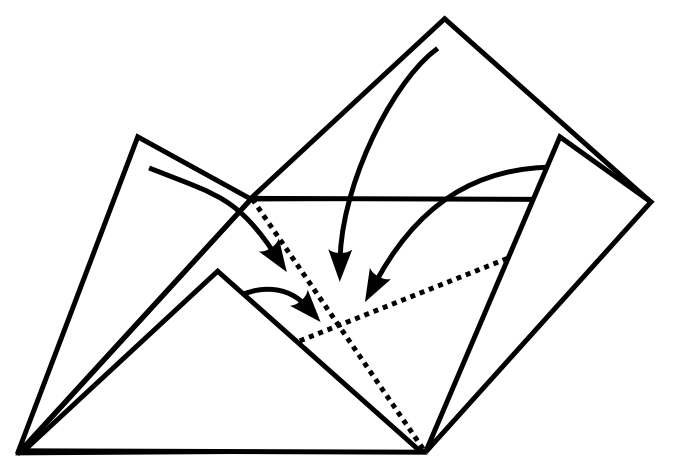
\includegraphics[width=2in]{fold}

\vskip -.9in {\gr One option is to just take \\repeated random samples.
\\
It is better to `fold' your data.}

\vskip 1cm
$\bullet$ Sample a random ordering of the data \\ { ~~(important to avoid order dependence)}

\vskip .1cm $\bullet$ Split the data into $K$ folds: { 1st 100/K\%, 2nd 100/K\%, etc}.

\vskip .1cm 
$\bullet$ Cycle through $K$ CV iterations with a single fold left-out.

\vskip .25cm
This guarantees each observation is left-out for validation, \\and lowers the sampling variance of CV model selection.

\vskip .25cm
Leave-one-out CV, with $K=n$, is nice but takes a long time.\\
$K=5$ to $10$ is fine in most applications.

\end{frame}


\begin{frame}
{CV Lasso}

The lasso path algorithm minimizes $-\frac{2}{n}\log\text{LHD}(\bs{\beta}) + \lambda_t \sum_j |\beta_j|$ over the sequence of penalty weights $\lambda_1 > \lambda_2 \ldots > \lambda_T$.

\vskip .25cm
This gives us a path of $T$ fitted coefficient vectors, 
$\nv \bs{\hat\beta}_1 \ldots \bs{\hat\beta}_T$,
each defining deviance for new data: $\nv -\log \text{p}(\bm{y}^{new}\mid\bm{X}^{new}\bs{\hat\beta}_t)$.

\vskip .5cm
Set a sequence of penalties $\lambda_1 \ldots \lambda_T$.  \\
Then, for each of $k=1\ldots K$ folds,
\begin{itemize}
\item Fit the path $\nv \bs{\hat\beta}^k_1 \ldots \bs{\hat\beta}^k_T$ on all data {\it except} fold $k$.
\item Get fitted deviance {\it on left-out data}: 
$\nv -\log \text{p}(\bm{y}^{k}\mid\bm{X}^{k}\bs{\hat\beta}_t)$.
\end{itemize}

This gives us $K$ draws of OOS deviance for each $\lambda_t$.

\vskip .5cm
Finally, use the results to choose the `best' $\theme \hat\lambda$, then re-fit the model to {\it all of the data} 
by minimizing $-\frac{2}{n}\log\text{LHD}(\bs{\beta}) 
+ {\theme \hat \lambda} \sum_j |\beta_j|$.

\end{frame}


\begin{frame}[fragile]
{CV Lasso}

{Both {\tt gamlr} and {\tt glmnet} have functions to wrap this all up.}

The syntax is the same; just preface with {\tt cv.}

\begin{semiverbatim}\nv
cv.spender <- cv.gamlr(xweb, log(yspend))
\end{semiverbatim}

Then, {\nv\tt coef(cv.spender)} gives you $\bs{\hat\beta}_t$ at the `best' $\lambda_t$
\begin{itemize}
\item {\tt select="min"} gives $\lambda_t$ with {\it min average OOS deviance}.
\item {\tt select="1se"} defines best as {\it biggest $\lambda_t$ with average OOS deviance no more than 1SD away from the minimum.}
\end{itemize}

\vskip .2cm
{\tt 1se} is default, and balances prediction against false discovery.  

{\tt min} is purely focused on predictive performance.

\end{frame}


\begin{frame}
{CV Lasso}

\vskip .25cm

Again, the routine is most easily understood visually.

\vskip -.25cm
\begin{center}
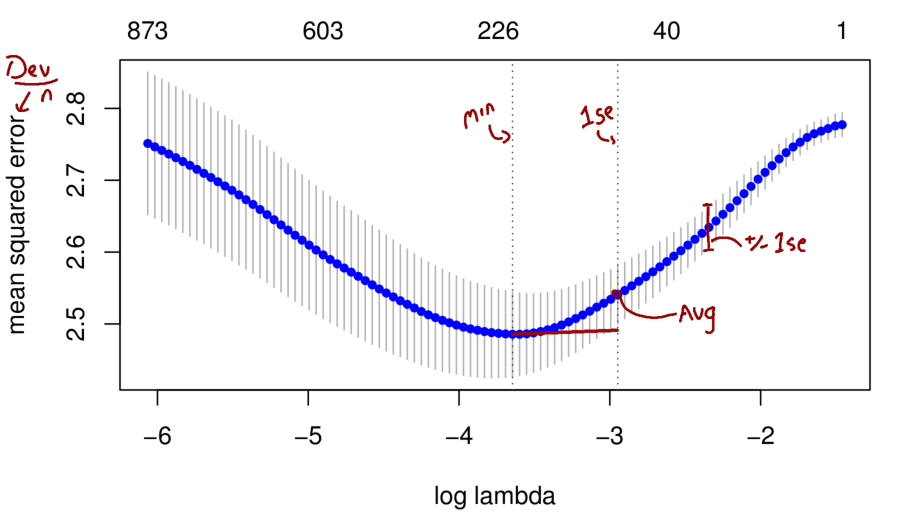
\includegraphics[width=\textwidth]{comscore_cvmarkedup}
\end{center}

\vskip -.25cm
Both selection rules are good; {\tt 1se} has extra bias for simplicity.
\end{frame}

\begin{frame}

{\Large Problems with Cross Validation}

\sk \nv It is time consuming:
{\bk When estimation is not instant, \\
fitting $K$ times can become unfeasible even $K$ in 5-10. }

\sk It can be unstable: {\bk imagine doing CV on many different samples.  
There can be large variability on the model chosen.}

\sk \bk Still, some form of CV is used in most DM applications.

\vskip .5cm {\gr Also, be careful to not cheat:} {\gr for example, with the FDR cut model we've
already used the full $n$ observations to  select the 25 strongest
variables.  It is not surprising they do well `OOS'.}

{The rules: if you do something to the data, do it {\it inside} CV.}

\end{frame}



\begin{frame}[fragile]
{\gr Alternatives to CV: \bk Information Criteria}

\vskip .25cm
{Many `Information Criteria' out there: AICc, AIC, BIC, ...}

These approximate distance between a model and `the truth'.

You can apply them by choosing the model with minimum IC.

\sk
Most common is Akaike's {\theme AIC = Deviance + $2df$.}

\vskip .2cm
$df$ = `degrees of freedom' used in your model fit.

For lasso and MLE, this is just the $\#$ of nonzero $\hat\beta_j$.

\vskip .5cm
For example, the {\tt summary.glm} output reports
\begin{semiverbatim}\small\nv
    Null deviance: 731.59 on 1476 degrees of freedom
Residual deviance: 599.04 on 1451 degrees of freedom\theme
AIC: 651.04
\end{semiverbatim}
and many recommend picking the model with smallest AIC.
{\gr Note the {\tt d.o.f.} in R output is `d.o.f. left after fit': $n-df$.}

\end{frame}

\begin{frame}
{AIC overfits in high dimensions}

The AIC is atually estimating OOS deviance: 
what your deviance would be on another {\it independent} sample of size $n$.

\vskip .5cm
IS deviance is too small, since the model is tuned to this data.  \\Some deep theory shows that IS - OOS deviance $\approx 2df$.
\vskip .1cm

\hskip 2in $\Rightarrow \text{AIC} \approx$ OOS deviance.

\sk
Its common to claim this approx (i.e., AIC) is good for `big $n$'.

{\theme Actually, its only good for big $n/df$. } 

\sk
In Big Data, $df$ (\# parameters) can be huge.  Often $df\approx n$.

In this case the AIC will be a bad approximation: it overfits!

\end{frame}

\begin{frame}
{AIC corrected: \nv AICc}

AIC approximates OOS deviance, but does a bad job for big $df$.
 
\sk
In linear regression an improved approx to OOS deviance is
\[
\theme \text{AICc} { ~\gr = \text{Deviance} + 2df\ds{E}\left[\frac{\sigma^2}{\hat \sigma^2}\right]} = \text{Deviance} + 2df\frac{n}{n-df-1}
\]
This is the corrected AIC, or AICc.  

\vskip .05cm
{It also works nicely in logistic regression, or for any {\tt glm}.}

\vskip .5cm
Notice that for big $n/df$, AICc $\approx$ AIC. So {\it always} use AICc.

\end{frame}

\begin{frame}[fragile]
{gamlr uses AICc}

\vskip .25cm

{It's marked on the path plot}

\vskip .25cm
\hskip .5in 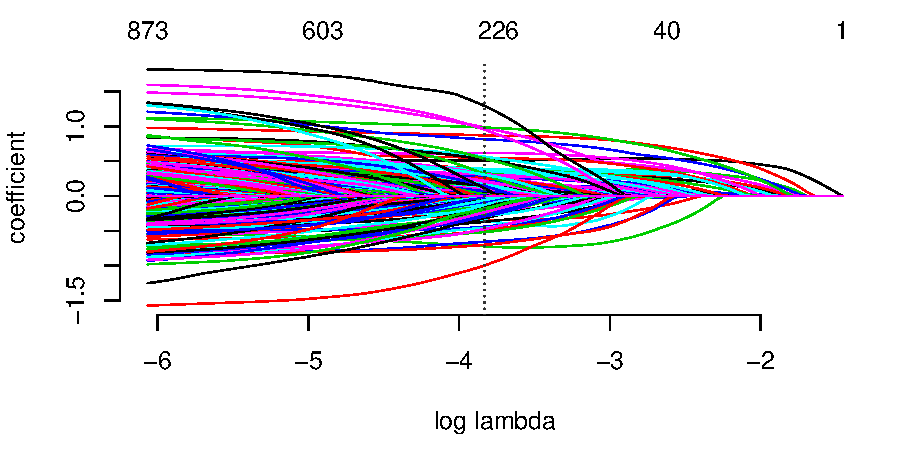
\includegraphics[width=.8\textwidth]{comscore_pathaicc}

\vskip .1cm
And it is the default for {\tt coef.gamlr}

\begin{semiverbatim}\nv\small
B <- coef(spender)[-1,] 
B[c(which.min(B),which.max(B))]\bk
    cursormania.com shopyourbargain.com 
          -0.998143            1.294246 
\end{semiverbatim}

\end{frame}

\begin{frame}
{{\gr Another option: } Bayes IC}

The BIC is  {\nv Deviance + $\log(n)\times df$}.

\vskip .05cm
This {\it looks} just like AIC, but comes from a very different place.

\vskip .25cm
$BIC \approx -\log \mr{p}(M_b|\mr{data})$, the `probability that model $b$ is true'.
\[
\mr{p}(M_b|\mr{data}) = \frac{\mr{p}(\mr{data}, M_b)}{\mr{p(data)}} 
\propto \gr\underbrace{\bk\mr{p}(\mr{data}|M_b)}_\text{LHD}
\underbrace{\bk\mr{p}(M_b)}_{\text{prior}}
\]
The `prior' is your probability that a model is true {\it before} you saw any data. {\gr BIC uses a `unit-info' prior: 
$\mr{N}\!\left[\bs{\hat\beta}, \frac{2}{n}\mr{var}(\bs{\hat\beta})^{-1}\right]$}

\vskip .25cm
AIC[c] tries to approx OOS deviance.\\
 BIC is trying to get at the `truth'.


\end{frame}

\begin{frame}
{IC and CV on the Comscore Data}

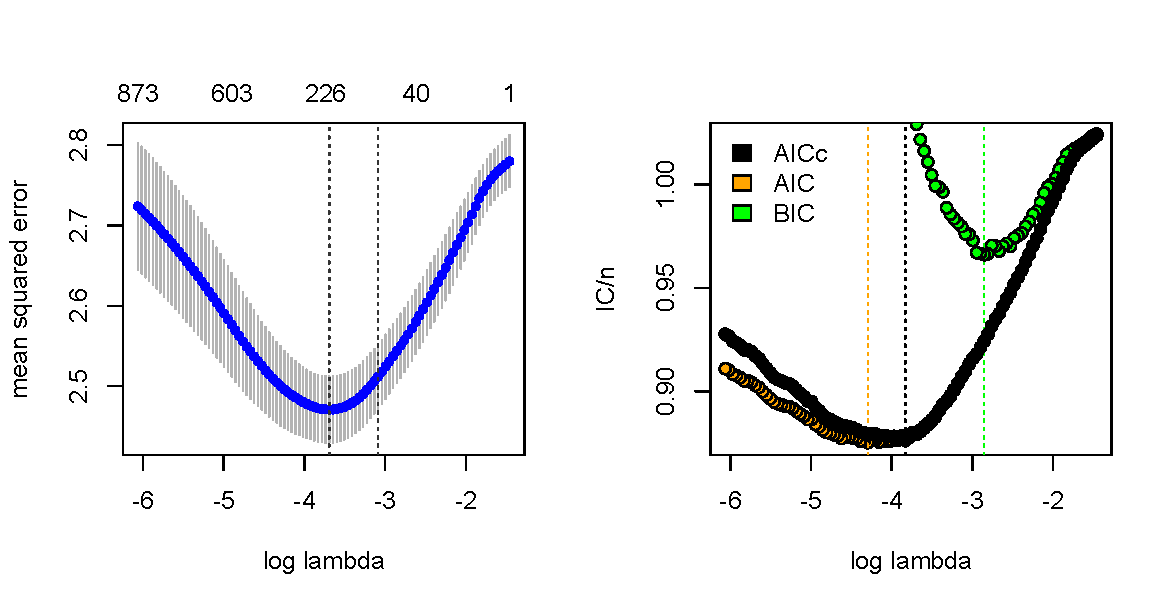
\includegraphics[width=\textwidth]{comscore_icvcv}

\sk
The take home message: AICc curve looks like CV curve.

 \vskip .25cm
In practice, BIC works more like the 1se CV rule.  \\
But with big $n$ it chooses too simple models (it underfits).

\end{frame}


\begin{frame}
{IC and CV on the Comscore Data}

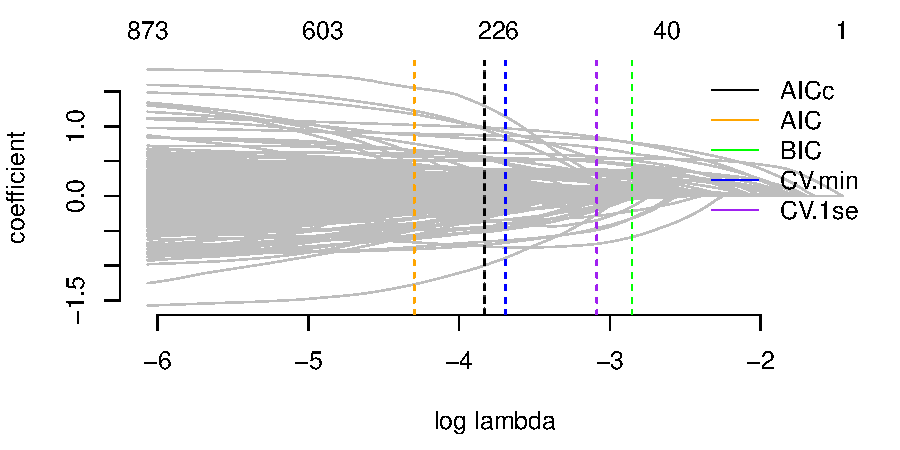
\includegraphics[width=\textwidth]{comscore_pathallic}

\vskip .2cm
With all of these selection rules, you get a range of answers.

If you have time, do CV.  But AICc is fast and stable.

If you are worried about false discovery, tend towards BIC/1se.

\end{frame}

\begin{frame}

\vspace{-.5in}
\begin{adjustwidth}{-.4in}{}

\includegraphics[width=5.1in]{../graphs/stickonpuck.jpg}

\vskip .6cm
{\bf ~~~~~{\theme Hockey Homework:} what are individual players contributing?}
\end{adjustwidth}

\vskip .25cm
A stat for player performance is the `plus-minus' ({\nv PM}).  \\
PM is a function of goals scored while that player is on the ice: \\{\nv \hfill the number of goals for his team, minus the number against.}

\vskip .25cm
 There is no accounting
for   teammates or opponents. \\
{\gr Due to `line matching' this could make a big difference.}

\vskip .25cm
Can we build a better performance metric with regression?

\end{frame}


\begin{frame}
{Hockey Regression}

Response is a binary 1 if home goal, 0 if away goal.  \\Home players get an x-value of {\tt +1}, and away players
 {\tt -1}. \\
Everyone off the ice is zero.
\[\nv
\begin{array}{cc}
~& 
\text{players (onice)}\\
\text{home~goal?} & {\tt AARON\_DOWNEY} ~~~\ldots\ldots\ldots~~~~
{\tt ZIGMUND\_PALFFY}\\
1& 1\hspace{1cm}\ldots~~~0~~-1~~0~~~\ldots \hspace{1cm} 0
\end{array}
\]

Our logistic regression plus-minus model is 
\[\nv
 \log \frac{\mr{p}(y=1)}{1-\mr{p}(y=1)} = 
\beta_0 +
\!\!\!\!\sum_{\tt home players}\!\!\!\!\beta_j ~~- \!\!\!\!\sum_{\tt away players}\!\!\!\beta_j
\]
$\beta_j$ is $j^{th}$ player's  partial effect:  When a goal is scored and player $j$ is on ice,
odds are multiplied by $e^{\beta_j}$ that his team scored.

\end{frame}


\begin{frame}
{Hockey Regression}

In addition to `controlling' for the effect of who else is on the ice, we also want to control for things unrelated to player ability. \\
{\gr (crowd, coach, schedule, ...)} 

\vskip .25cm
 We'll a `fixed effect' for each team-season, $\alpha_{team,season}$.

\vskip .1cm
Also, special configurations (e.g., 5 on 4 power play) get 
$\alpha_{config}$.

\vskip .1cm
So the full model has `{\it log odds that a goal was by home team}'
\[\nv
\beta_0 + \alpha_{team,season} + \alpha_{config} +
\!\!\!\!\sum_{\tt home players}\!\!\!\!\beta_j ~~- \!\!\!\!\sum_{\tt away players}\!\!\!\beta_j
\]

{\tt gamlr} includes data on NHL goals from 2002/03-2012/13.\\
The code to design and fit this model is in {\tt hockey\_start.R}.\\
Via the {\tt free} argument, only player $\beta_k$'s are penalized.

\end{frame}

\begin{frame}
{Homework due next lecture}

[1] Interpret AICc selected model from my {\tt nhlreg} lasso. \\ Just tell some stories about what the model tells you.

\vskip .25cm
[2] The {\tt gamlr} run for {\tt nhlreg} uses {\tt standardize=FALSE}.
Why did I do this?  What happens if you {\it do} standardize?

\vskip .25cm
[3] Compare model selection methods for the {\tt nhlreg} lasso.  Consider both IC and CV  (you'll want to create {\tt cv.nhlreg}).

\vskip .25cm
[4] We've controlled our estimates for confounding information from team effects and special play configuration.  How do things change if we ignored this info (i.e., fit a player-only model)?  Which scheme is better (interpretability, CV, and IC)?

\vskip .25cm\gr
[+] Can you translate player $\beta_k$ effects into something comparable to classic Plus-Minus?  How do things compare?

\end{frame}


\end{document}